\documentclass{article} \usepackage{tabularx}
\usepackage{amsmath} \usepackage{amssymb} \usepackage{tikz}
\usepackage{booktabs}
\usepackage{float} \restylefloat{table} \graphicspath{{images/}}
\usepackage[margin={3.5cm,3cm}]{geometry} \usepackage{multicol}
\setlength\columnsep{1.5cm} \usepackage{tabto}
\usepackage{pdflscape} \usepackage{graphicx} \usepackage{array}
\usepackage[T1]{fontenc} \usepackage[utf8]{inputenc}
\usepackage{charter} \usepackage{environ} \usepackage{tikz}
\usetikzlibrary{calc,matrix}
% For citations
\usepackage[sort,numbers]{StyFiles/natbib}
\renewcommand{\citename}{\citet} \renewcommand{\cite}{\citep}
\usepackage{StyFiles/natbibspacing}


\begin{document}


\begin{titlepage}
	\centering
	\begin{figure}[H]
    \centering
    % \includegraphics[scale=0.5]{logo_nasa_trio_black@2x.png}
	\end{figure}
	\vspace{2cm} {\scshape\LARGE Literature Review\par}
  \vspace{2cm}
  
  %%%%%%%%%%% Title
	{\scshape\LARGE

    Sequence Learning Using Deep Neural Networks With Flexibility
    \& Interpretability
    
    \par} {\huge\bfseries \par}
	
	\vspace{2cm} {\Large\itshape Chang \textsc{Li}\par} \vfill

  {\Large Supervisor\par} {\Large\itshape Prof. Dacheng
    \textsc{Tao}\par} \vfill

\end{titlepage}


\section{Introduction}
\label{sec:intro}

One interesting task in machine learning is modeling complex
sequences having long-term dependencies. Many applications such
as machine translation, complex dynamical system analysis,
activity recognition and behavioral phenotyping tools for
neuro-science involved with capturing non-linear patterns in
sequences. Sequence learning mainly have three difficulties:
approximating non-linear relationship among sequences, feature
selection and capturing long-term dependencies. Our primary aim
of this proposal is mainly focused on demonstrating those three
difficulties. 

Despite substantial effort has been made for modeling sequences,
many of those models are either unable to approximate non-linear
relationships or have rigid assumptions due to the dependency on
predefined form of prior function. For example, autoregressive
moving average (ARMA) model~\cite{hibon1997arma} cannot capture
non-linear relationships. Probabilistic Graphical
Models~\cite{murphy2012machine,koller2009probabilistic} (PGMs)
are very well studied for the past decades. However, capabilities
of approximating non-linear patterns of PGMs are also severely
suffered from rigid assumptions over priors.

Deep Neural Networks~\cite{goodfellow2016deep} (DNNs) are
powerful and flexible models that have outperforming performance
on various difficult learning tasks. Despite the powerful
capability of approximation, one significant limitation of DNNs
is that they require fixed dimension of inputs and targets.
\citename{sutskever2014sequence} in 2014 demonstrated this
difficulty as sequence to sequence problems. They introduced an
encoder-decoder framework based on two Recurrent Neural Networks
(RNNs) and achieved a very successful result in machine
translation. The key ideas (as shown in Figure~\ref{fig:en-de})
behind encoder-decoder networks and its variants are that they
first encode the whole sentence of words into a single, fixed
length variable using encoder network. Then a decoder network is
used to decode that variable and generate translation. One major
drawback is that ``indeed the performance of a basic
encoder–decoder deteriorates rapidly as the length of an input
sentence increases~\cite{attention}''. Since for many sequence
learning applications there exists many long-term dependencies
relationships, the question of solving this drawback remains
open.

\begin{figure}[H]
  \centering
  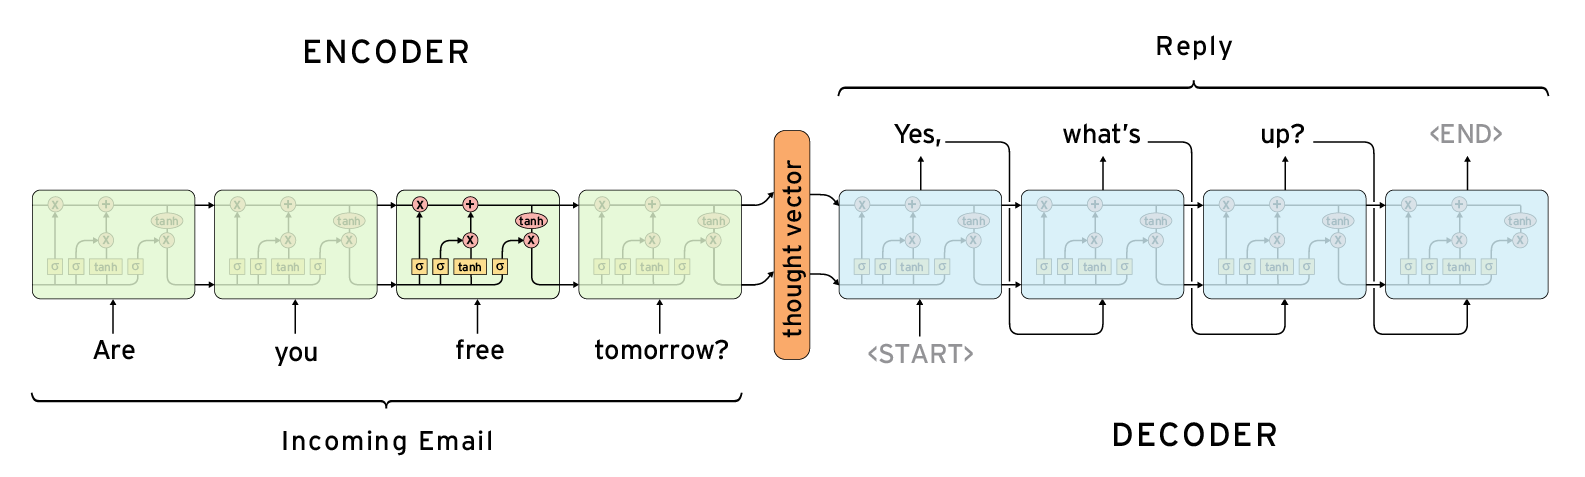
\includegraphics[scale=0.5]{images/en-de.png}
  \caption{Encoder-Decoder Network}
  \label{fig:en-de}
\end{figure}

Other than long-term dependencies difficulty, DNNs contain a very
large number of latent variables which make the training results
very hard for a human to interpret~\cite{goodfellow2016deep}.
Being able to explain the reasons behind such models plays a
crucial role in tasks such as model comparison and deployment. It
could also provide insights into the data set and model itself.
Thus improving the interpretability of DNNs could also be a very
interesting topic to investigate.

\section{CapsNet: Novel Interpretable Knowledge Representation
  Techniques}
\label{sec:caps_intro}

Neural networks have shown dominant advantages of extracting
features and recognizing patterns from raw data directly without
domain knowledge over conventional statistical methods. One of
the most successful architecture, CNNs, achieves the ability of
classifying objects without prior knowledge of positioning by
creating a pool of neuron activities and down sampling the most
active scalar from the pool. It also use convolution operation to
replicate knowledge through different positions. Together with
multi layer structure, CNNs achieves translational invariance and
viewpoint invariance. However, one problem of CNNs is the missing
information about pose (position, size, orientation) matrix of
entities during the procedure of down sampling. While
facilitating CNNs achieving viewpoint invariance, lacking of pose
information also leads to several severe problems such as
vulnerable to adversarial attacks, incapable of overlapping
objects recognition and 3D objects recognition.

In 2017, \citeauthor*{capsule}\cite{capsule} revives an ancient
technology, the capsule neural networks, to tackle these
difficulties. The origination of capsule neural networks can be
tracked down to 1980s when it is first introduced as a feature
extracting technology which achieves viewpoint invariance in task
of recognizing constellations \cite{zemel1990traffic}. In that
paper \citeauthor*{zemel1990traffic} \cite{zemel1990traffic}
discovered that using a vector of parameters as output of neurons
instead of a single scalar shows some promising properties such
as viewpoint invariance. However subjected to computational
difficulties at that time, they were unable to prove the
effectiveness of this method and could not develop a mature
method utilizing the nice feature extracted by capsules forming
more abstract entities.

More than 20 years later, in 2011 a group of authors
\citeauthor*{hinton2011transforming}
\cite{hinton2011transforming} re-discovered this method and were
able to show the feature extracted by capsules can be easily
trained to learn the pose parameters from pixel intensities. The
remaining task of capsule neural networks is simply finding a
grouping method which can translate the lower entities' knowledge
to higher entities in order to formulate a part-whole
relationship between capsules.

\citename{capsule} followed this by developing a so called
``routing by agreement'' iterative method to route knowledge
learned by lower layer capsules to higher layers capsules
according to lower layer capsules' agreement.
\citename{hinton2018matrix} extended this method by designing a
EM like algorithm which treats higher layer capsules as Gaussian
distributions and lower layer capsules as data points. The
routing problem then becomes a Gaussian Mixture Model (GMM)
clustering problem by assigning lower layer capsules (data
points) to higher layer capsules (Gaussian).

Here we will briefly examine the development of the capsule
neural networks and how those methods are relevant to our
research.

\subsection{Instantiation Parameters Extracting}
\label{sec:instan}

One advantage of CNNs is the viewpoint invariance property
achieved by using down sampling method. The main difficulty comes
with it is that the missing information of pose matrix.
\citename{zemel1990traffic} argued that instead of using a scalar
as the output of neuron, we could use a more complex mechanism to
organize neurons in a more organized way and outputs a vector of
real values to encode the pose information. They also separated
the task of extracting features from image intensities into two
subtasks. They represent the knowledge of entities themselves
into a vector of instantiation parameters (neuron activities)
which is equivariant with respect to viewpoint changes in raw
images. And encode the knowledge of part-whole relationships
using weight matrix which is viewpoint invariant and can be
learned during the end-to-end training.

They proved this by utilizing the fact that the reference frame
of all parts of an entity should produce identical reference
frame (the entity's) after transformation (the ``viewpoint
consistency constraint''). In their configuration, there are two
layers of neurons. Neurons in lower layer represents features
extracted from raw images. Each feature (capsule) is composed of
a vector of real values which can be seen as the flatten version
of the pose matrix. Neurons in higher layer represents more
abstract objects which also contains a vector of real values as
instantiation parameters. Therefore, the fixed transformation
matrix which describes the structural relationship between
features and objects can be encoded in the connectionist network
as the weight matrix between those two layers.

Let $T_{fo}$ be the transformation matrix from object to feature
frame, $T_{io}$ be the transformation matrix from object to
image frame and $T_{if}$ be the transformation matrix from
feature to image frame. Then we have the equality that

$$T_{io}=T_{if}T_{fo}$$

Therefore once we learned from the feature-object pair to get
$T_{fo}$ and got $T_{if}$ from raw input image, the
transformation matrix $T_{io}$ can be easily computed by simply
multiply those two matrix.

Therefore, suppose the instantiation parameters of capsules at
lower layer are represented as $P_{if} =
(x_{if},y_{if},c_{if},s_{if})$ in which the first two parameters
are coordinates. $c_{if}$ is the scale and $s_{if}$ is the angle
of the feature frame. Accordingly, we can use $P_{io} =
(x_{io},y_{io},c_{io},s_{io})$ to represent the object frame and
$P_{fo} = (x_{fo},y_{fo},c_{fo},s_{fo})$ to represent the object
to feature frame. We can easily represent the transformation
matrix from feature frame to image frame by using:

\begin{align*}
  T_{if}=
  \begin{bmatrix}
    c_{if} & s_{if} & x_{if} \\
    -s{if} & c_{if} & y_{if} \\
    0 & 0 & 1
  \end{bmatrix}
\end{align*}

Under this formulation, the reference frame transformation
between lower layer features (parts of entity) and higher layer
objects (more abstract entity) can be encoded in the weight
matrix between two layers and can be learned end-to-end from the
training algorithm. This novel formulation results a very nice
property that the weight matrix which represents the structural
relationship between part and whole is viewpoint invariance while
the instantiation parameters which are represented neuron
activities are equivariant to the viewpoint changes of entities
in raw images.

Following their work, \citename{hinton2011transforming} for the
first time gave a formal definition of the capsule neural
networks and demonstrated its capability of extracting explicit
pose information from raw image intensities inputs.

\begin{figure}[H]
  \centering
  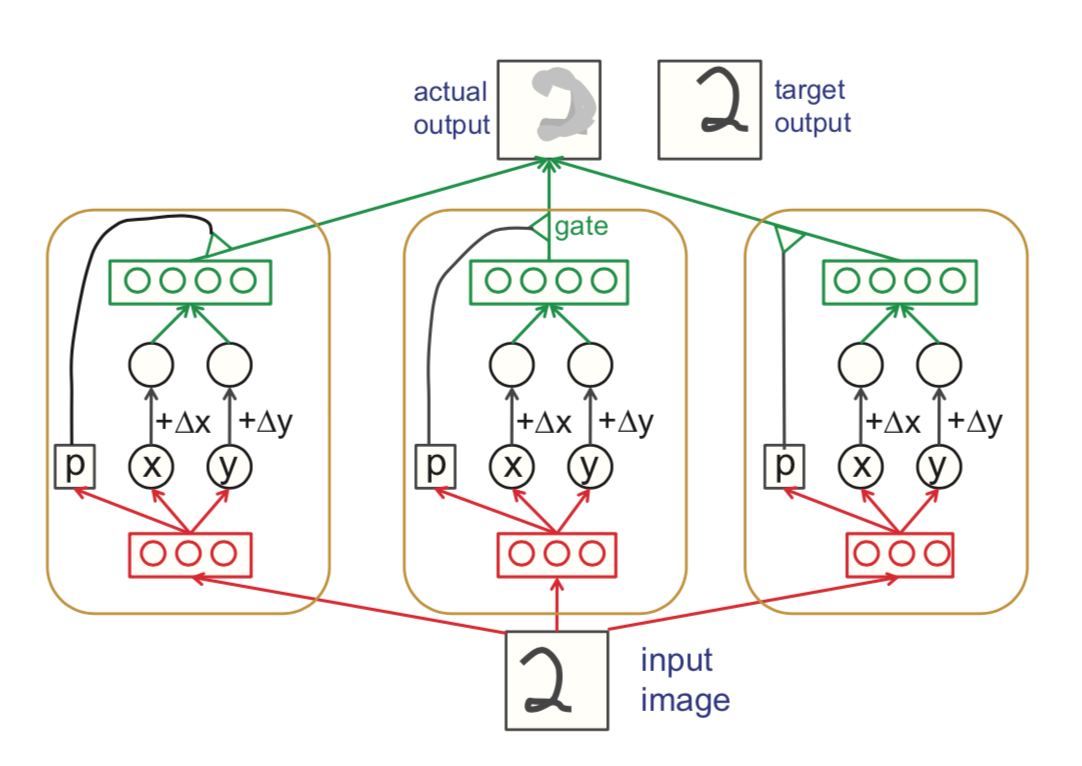
\includegraphics[scale=0.5]{images/caps_cord.png}
  \caption{Capsules in Transforming Auto-encoders}
  \label{fig:caps-cord}
\end{figure}

As can be seen in figure~\ref{fig:caps-cord}, each capsule
contains two sub layers. The neurons in lower layer are called
``recognition units'', which receive raw image intensities as
inputs and outputs three values. Values $x$ and $y$ are simply
the coordinates of the entity that capsule represents. The value
$p$ measures the degree of existence of the entity in the
original image. This measure can be viewed as the probability of
the entity appears in the image. 

The task of this paper is to reconstruct the shifted image from
the input image. \citename{hinton2011transforming} argued that
similar to human brain receives fixation movements from eyebrow
movements, the neural net neurons could also have direct
transformation information to facilitate the prediction of
coordinates of the shifted image. Therefore following the
recognition units, the shift information $\Delta x$ and $\Delta
y$ are added directly to the outputs and then be used as inputs
to the higher sub-layer. The higher sub-layer is called
``generation units'' which is also composed of a vector of
neurons. Neurons in this layer are simply like conventional
neurons which make predictions of the inputs. One subtle thing is
that instead of directly passed to higher layer, outputs of
generation units are firstly multiplied with the probability
measurement $p$.

\begin{figure}
  \centering
  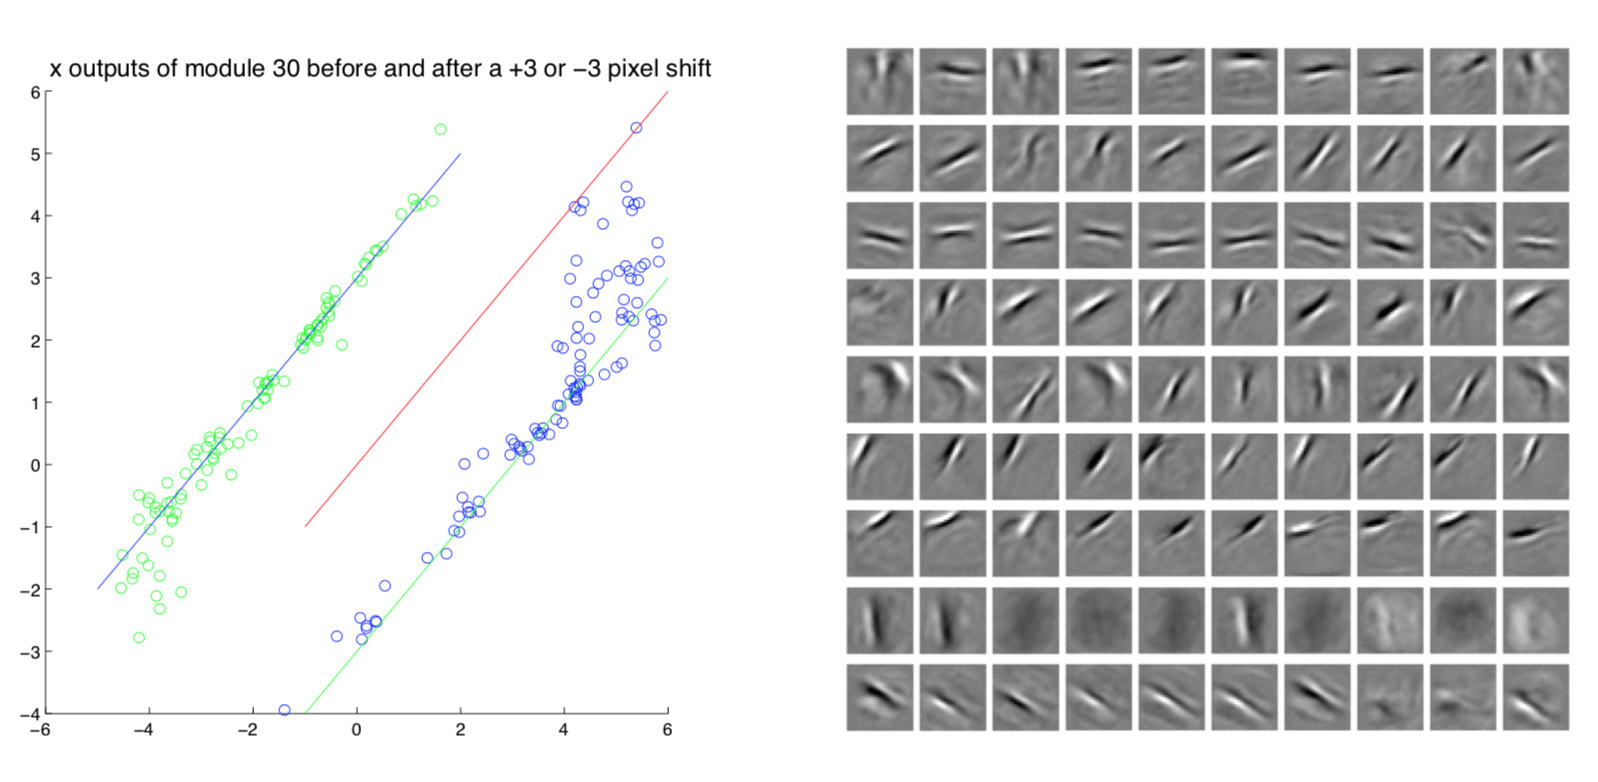
\includegraphics[scale=0.5]{images/trans_caps.png}
  \caption{Transforming Auto-encoders Result. The left image
    shows coordinates predicted by recognition units. The right
    image shows weight matrix of 10 generative units from 9
    capsules.}
  \label{fig:trans_enco}
\end{figure}


As a simple demonstration of capsule neural networks' capability
of learning pose information explicitly, the previous network
configuration was trained on randomly shifted images from MNIST
dataset. Results reported in their paper (see
figure~\ref{fig:trans_enco}) showed that for most of pixels
recognition units are able to predict the shifted coordinates
correctly. Exceptions appeared for border and corner pixels.
Generative units on the contrary can learn highly localized
weight matrix from recognition units' outputs which proved that
the effectiveness of capsule neural networks.

All of the above works are concentrated on the lower layer
configuration of capsule neural networks. They first proposed a
novel network architecture which use a group of neurons instead
of a single neurons as the output of one layer. The advantages of
viewpoint invariance achieved in weight matrix and viewpoint
equivariant in instantiation parameters were elaborated by using
reference frame and consistency constraint theory. Then they
proved the effectiveness of capsule neural networks extracting
pose information from raw image intensities.

At this stage, the task of recognition has been separated into
two concerns. One is extracting features directly from image
intensities which has been proved could be easily done using the
novel network architecture. The other is how to formulate the
part whole relationship, namely pass lower layer capsules'
information to higher layer capsules.

\subsection{Modeling Part-whole Relationship Between Capsules}
\label{sec:partwhole}

\citename{capsule} followed previous work on capsule neural
networks and extended the mechanism of pose information
extracting to object recognizing. The main difficulty they
demonstrated in that paper is how lower layer capsules' outputs
can be used to make contributions to higher layer capsules'
instantiation parameters.

In previous work \cite{zemel1990traffic,hinton2011transforming},
each lower capsule contributes to their parents (higher layer
capsules) individually by weighting their outputs with the
probability predicted. Parent capsule receives incoming values
from all of its children capsules and the instantiation
parameters is calculated by simply averaging all those incoming
values. This technique of sending lower layer information to
higher layer makes a strong assumption on the lower layers'
inputs that there will always exist strong enough good
predictions which can cancel other deviations at any degree.
Apparently this is not an ideal method.

\begin{figure}
  \centering
  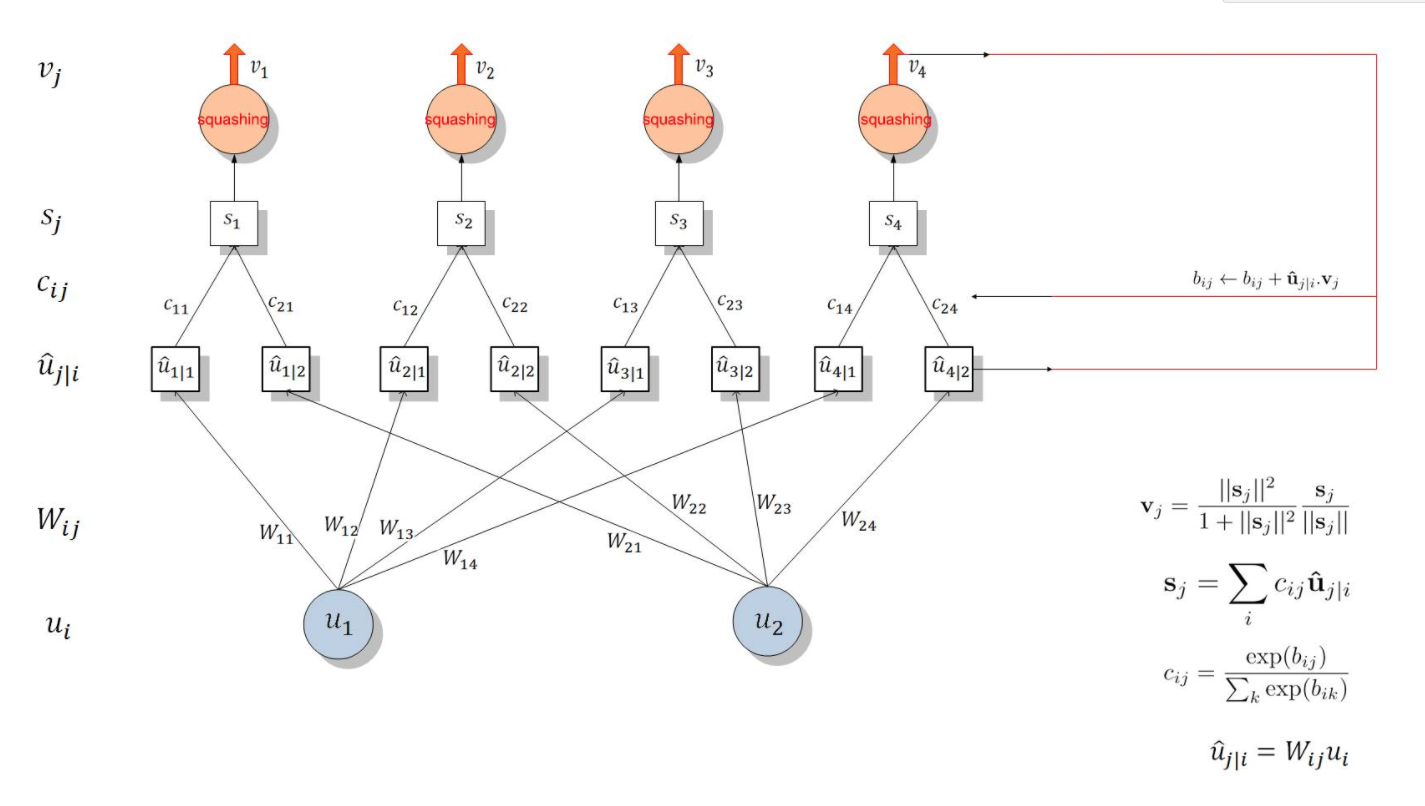
\includegraphics[scale=0.3]{images/capsnet_recursive.png}
  \caption{Dynamic Routing Architecture}
  \label{fig:routing}
\end{figure}

To tackle with this issue, \citename{capsule} proposed a type of
``routing-by-agreement'' algorithm. The architecture they used
for constructing capsule layers (see figure~\ref{fig:routing}) is
slightly different from previous works
\cite{zemel1990traffic,hinton2011transforming}. Instead of
outputs instantiation parameters together with the probability of
the existence of the entity that capsule represents in the image,
the capsule under their configuration only outputs a vector of
instantiation parameters. The entity is represented by the
orientation of the instantiation vector and the probability of
existence is represented by the length of it. By using this
formulation the routing path from lower layer capsules to higher
layer capsules can thus determined by comparing the dot product
between them. Information from lower layer capsules are only
routed to higher layer capsules which have large dot product
value with them.

To facilitate dynamic routing mechanism, there are also several
subtle techniques used in this work. As can be seen in
figure~\ref{fig:routing}, the configuration of lower layer
capsules are almost the same with previous works. Each lower
layer capsule $i$ outputs a instantiation vector $u_i$ which is
transformed by the weight matrix $\hat{u}_{j|i}=W_{ij}u_i$. The
variable $\hat{u}_{j|i}$ is called ``predictions'' made by lower
layer capsules. The transformation is identical to previous
works' which has a very nice property of viewpoint invariance.
However, the dimension of instantiation vector $u$ is much higher
than previous versions to encode various visual properties such
as pose, lighting and deformation etc.

The prediction vector $\hat{u}_{j|i}$ are then multiplied by a
coupling coefficient $c_{ij}$ which is dynamically updated by
``routing-by-agreement'' algorithm. The output $s_j$ is a
summation over all incoming lower layer capsules' prediction
vectors weighted by coupling coefficients. Because the length of
instantiation vector is used to predict the probability of
represented entity's existence, the variable $s_j$ is further
processed using a ``squanshing'' function which narrows the
distribution of the length close to zero and one.

The power of ``routing-by-agreement'' algorithm lies in the
iterative updating schema of coupling coefficient $c_{ij}$. As
can be seen in figure~\ref{fig:routing}, the coupling coefficient
is a softmax function over variable $b_{ij}$. The variable
$b_{ij}$ here acts like a log prior probability of the capsule
$i$ should make predictions to capsule $j$. In each iteration,
the log prior probability $b^{l+1}_{ij}$ is updated by addition
of previous $b^l_{ij}$ and the dot product of incoming capsule's
prediction vector $\hat{u}_{j|i}$ and instantiation vector of
parent capsule $v_j$. The dot product acts like a log likelihood
probability which measures the likelihood of capsule $i$ should
make predictions to capsule $j$ and thus be called the
``agreement'' between lower layer capsules and higher layer
capsules. By using this iterative schema, information contained
in lower layer capsules are only sent to higher layer capsules
which have strong agreement with the incoming prediction from it.

The result of ``routing-by-agreement'' mechanism is a part-whole
relationship parsing tree. Each node in the parse tree is an
activated capsule. The parents of that node is chosen by the
dynamic routing mechanism. Under this configuration, the network
architecture is not only viewpoint invariance in weight matrix
and equivariant in instantiation parameters, the classification
result is also a highly interpretative structure of part-whole
relationships.

\section{Sequence Learning Methods}
\label{sec:method}

\subsection{Modeling Long-term Dependencies And Feature
  Selection}
\label{sec:ltfs}

As discussed in section~\ref{sec:intro}, encoder-decoder networks
based on RNNs outperform many other statistical machine learning
models while suffering from short-term memories due to encoding
global information into a single fixed length variable. One of
the most popular ways is to introduce ``attention mechanism''
into encoder-decoder networks~\cite{attention}.

\citename{attention} demonstrated long-term dependencies issue by
introducing context vectors in the middle of encoder network and
decoder network (as shown in Figure~\ref{fig:attention}). Instead
of encoding the global information into a single variable,
attention mechanism enables encoder network to provide a sequence
of encoded vectors on which decoder network can do soft-searches.
As a result, decoder network is able to concentrate on the most
relevant information represented by a subset of encoded vectors
of arbitrary length. Thus encoder-decoder networks can have much
better performance when dealing with long-term dependencies.

\citename{qin2017dual} extended \citename{attention}'s work to
adaptively select most relevant hidden states as well as most
significant features simultaneously. They developed a dual stage
RNNs (see Figure~\ref{fig:darnn}). Other than attention vector
between encoder and decoder layer (so called ``Temporal attention
Layer'' in Figure~\ref{fig:darnn}(b)), they adaptively weights
input sequence $x_t^k$ which is the $k$th feature at $t$ step by
attention $\alpha_t^k$ (see Figure~\ref{fig:darnn}(a)). The input
attention mechanism is a feed-forward network. Thus the extended
encoder-decoder network can weight features according to their
importance while the whole network can still be trained jointly.
However, their work is focused on regression. We will further
investigate their methods by extending to classification cases.

\begin{figure}
  \centering
  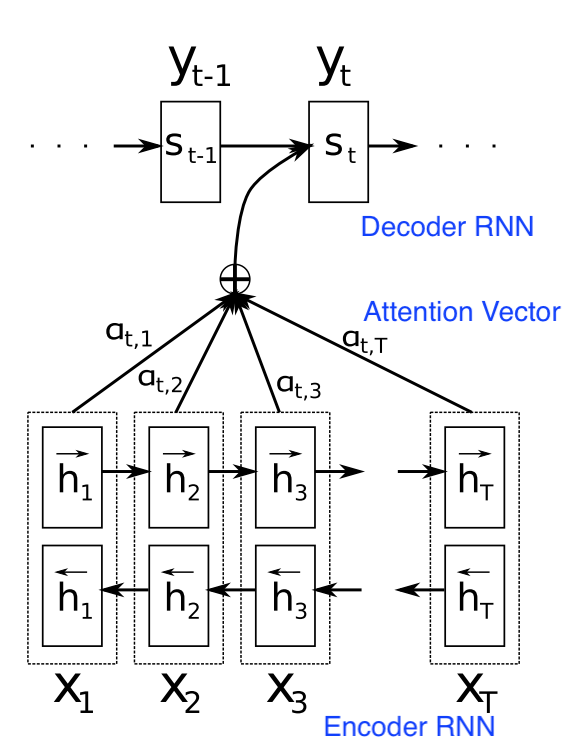
\includegraphics[scale=0.5]{images/attention.png}
  \caption{Attention Mechanism}
  \label{fig:attention}
\end{figure}

\begin{figure}[H]
  \centering
  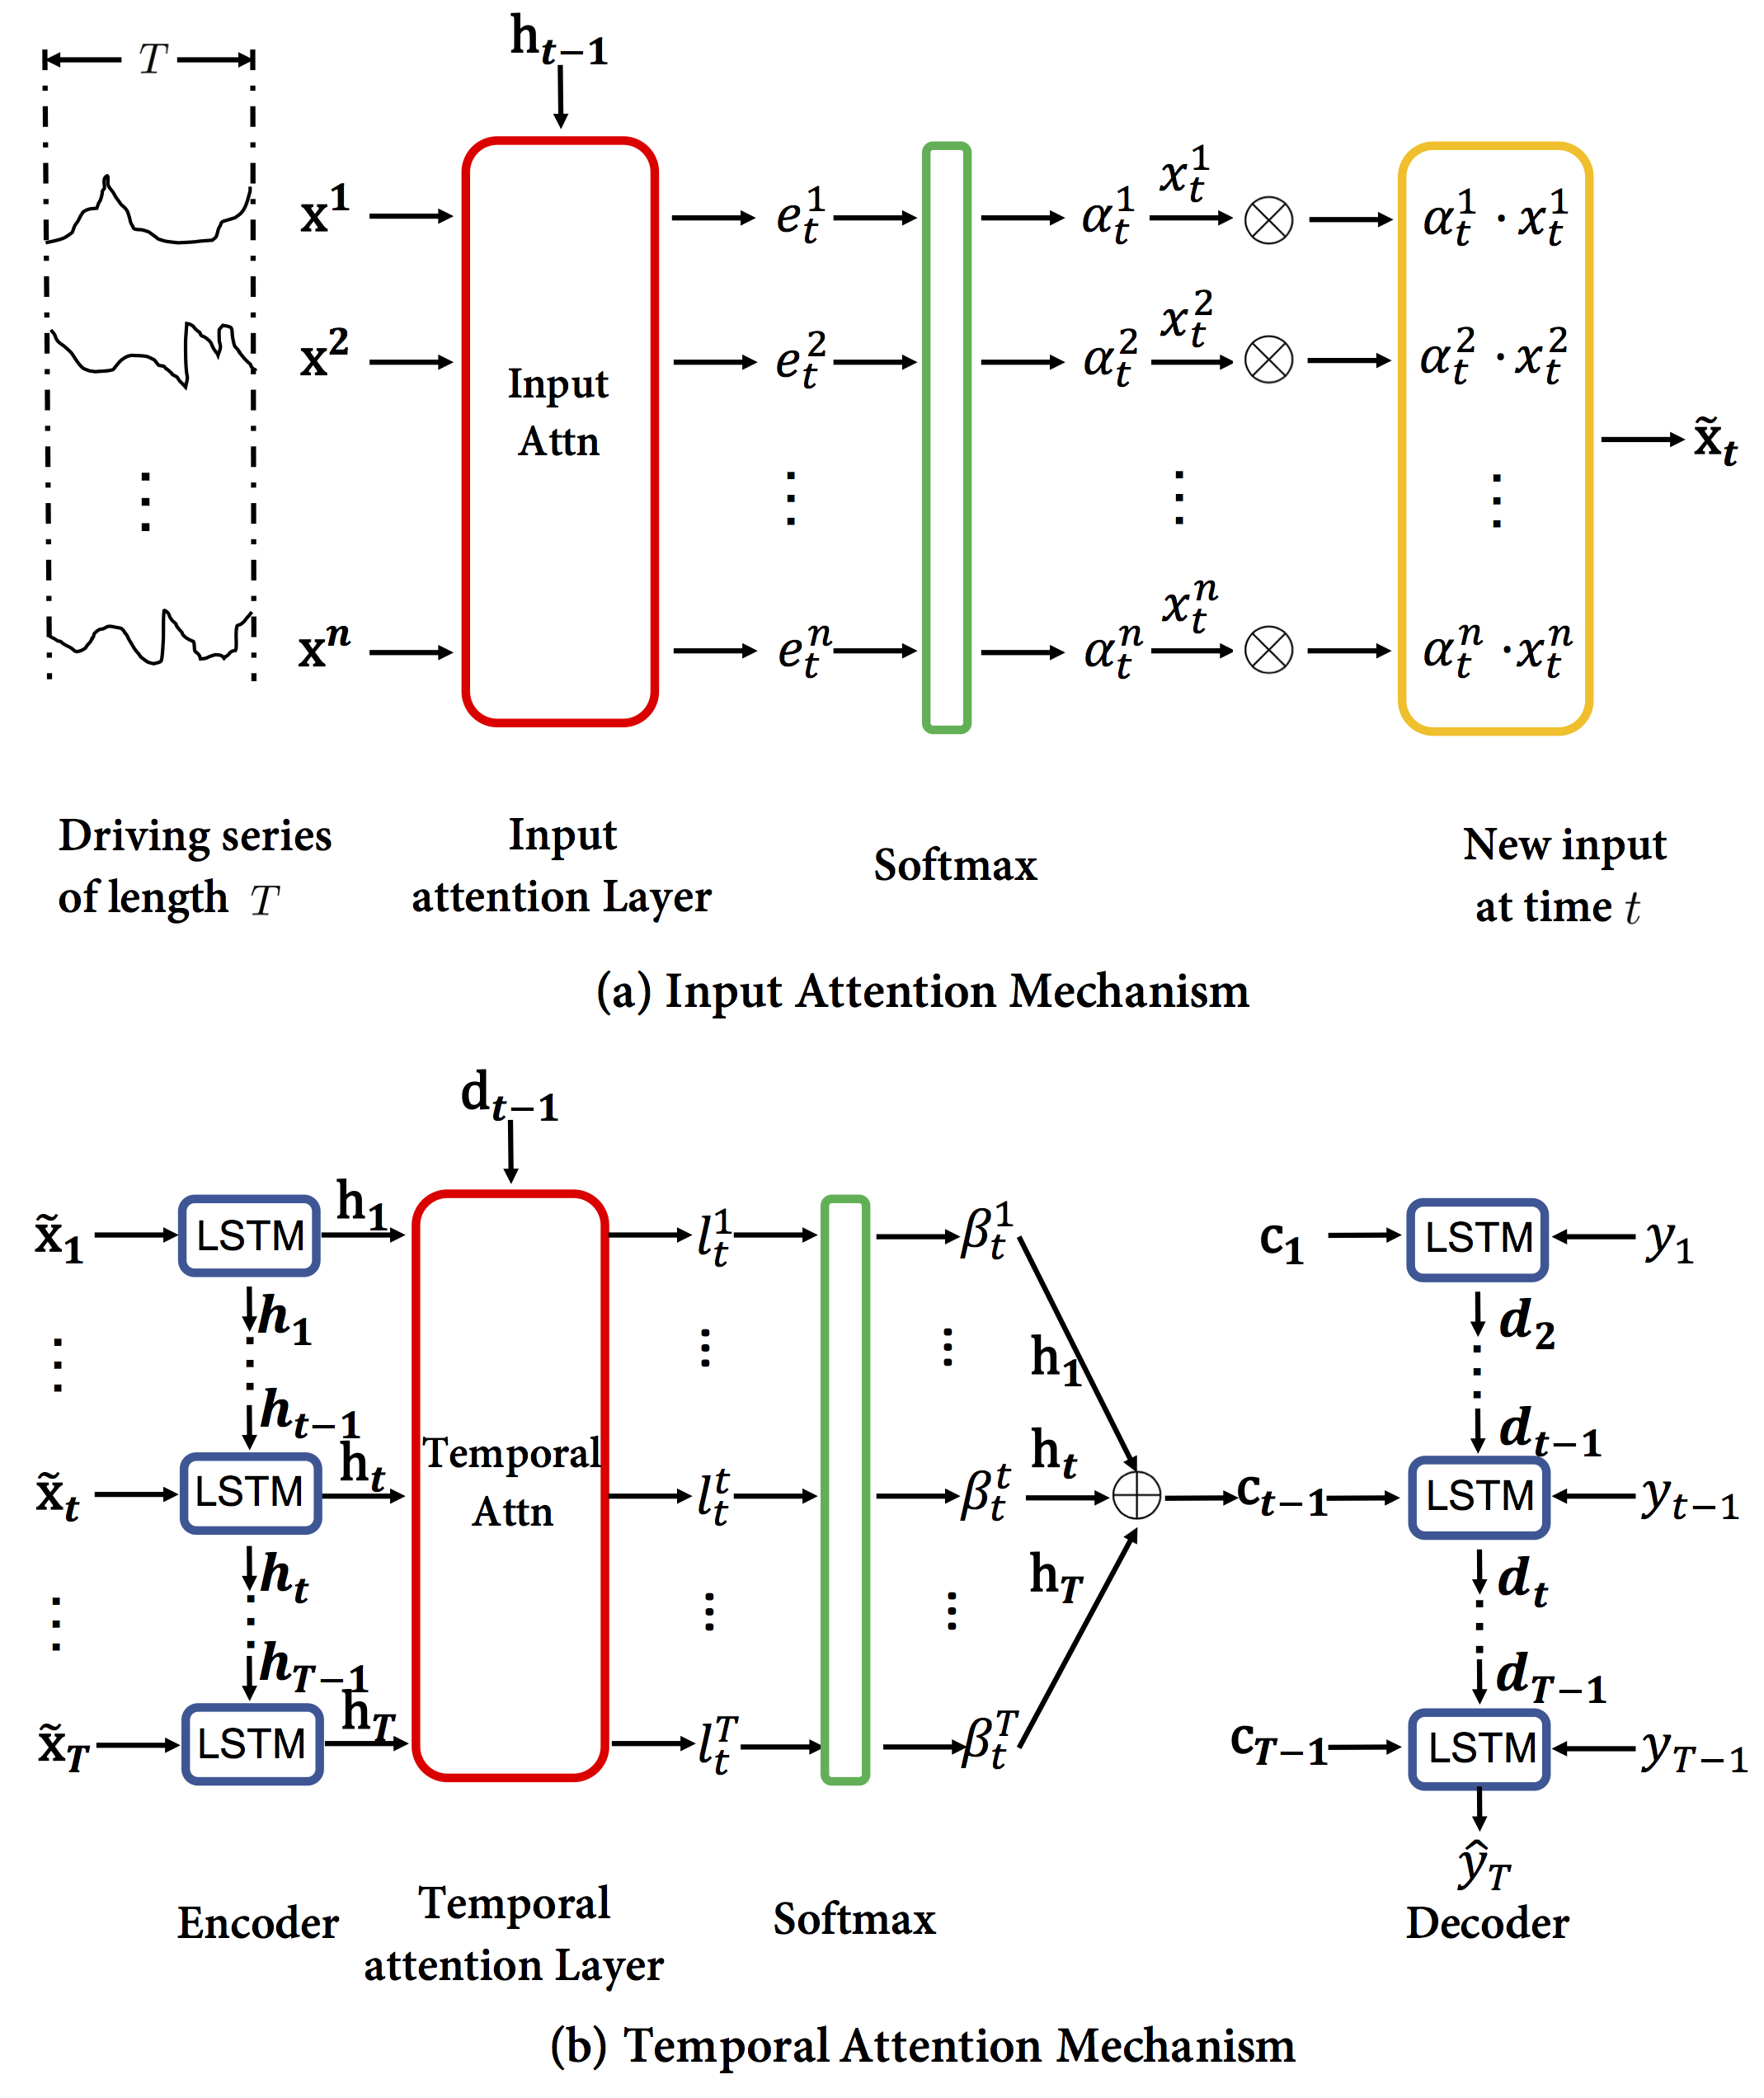
\includegraphics[scale=0.3]{images/darnn.png}
  \caption{Dual-Stage Attention Based RNN}
  \label{fig:darnn}
\end{figure}

\subsection{Topologies With Better Computational Properties}
\label{sec:better_comp}

One major drawback of RNNs is computationally expensive. RNNs
usually have a very deep recursive structure. It maintains hidden
states of the entire past which prevents parallel implementation
of the algorithm. On the contrary, Convolutional Neural Networks
(CNNs) have a hierarchical structure and can fully exploit the
GPU hardware by using parallel computing techniques.
\citename{gehring2017convolutional} attempted to replace RNNs
with CNNs in sequence modeling task by using a hierarchical
structure CNNs. They captured correlations in length of $n$
sequence by applying $\mathcal{O}(\frac{n}{k})$ convolutional
operations for kernels of width $k$ and constructed both of
encoder and decoder networks using CNNs. Results of their model
are slightly better than conventional encoder-decoder
networks~\cite{attention} on multiple data set but with a huge
decreasing in training time.

Recently, numerous pure attention architecture have been proposed
and achieved the state-of-the-art results in natural language
processing problems. \citename{vaswani2017attention} dispensed
CNNs and RNNs entirely and proposed a self-attention-based model.
They extends the conventional attention mechanism to a so-called
Multi-Head Attention (MHA) architecture by allowing each head to
generate different distributions over encoder output. This novel
network architecture has very concise topology representation and
outperforms both RNNs and CNNs based sequence to
sequence~\cite{vaswani2017attention} models.

In this project we plan to further investigate those network
topologies. Besides, the question of creating attention mechanism
in input layers (feature selection) in those architectures still
remains open.

\subsection{Interpretability}
\label{sec:interp}

Substantial effort has been made for improving DNNs
interpretability in recent years. There are mainly three
different types of approaches:

\begin{itemize}
\item Explain local predictions directly
\item Approximating DNNs using human interpretative models
\item Joint learning probabilistic graphical models with DNNs
\end{itemize}

\citename{ribeiro2016should} proposed a Local Interpretative
Model-agnostic Explanations (LIME) method to interpret arbitrary
machine learning models directly by explain individual outputs.
They tried to approximate a human interpretative local estimator
(Lasso in their case) by sampling around models' outputs and
explain the reason behind those decisions by observing which
features (input) are taking most responsibility in the local
estimator. However, such approaches are limited to providing
explanations for individual decision. A more challenging task
would be providing a global insights of models.

Instead of explaining local predictions, \citename{SDT} use the
DNNs to train a soft decision tree. One main difficulty of such
model is that it requires exponentially large amount of training
data with respect to the depth of the tree. However, with
approximated DNNs in hand, sufficient amount of training data for
soft decision tree can be provided by labeling unlabeled data
using DNNs, sampling synthetic unlabeled data using generative
approach~\cite{goodfellow2014generative} and distilling
method~\cite{hinton2015distilling}. Such soft decision tree could
approximate DNNs to a reasonable extent while maintain human
interpretability for further investigation.

More advanced approaches combines complementary strengths of
Probabilistic Graphical Models (PGMs) and DNNs.
\citename{johnson2016composing} proposed a combination of
flexible deep learning feature models with structured Bayesian
priors. They used deep auto-encoders to extract lower
representation of non-linear observed data and used graphical
models for latent variables sequence inference. A very efficient
variational inference algorithm was developed to solve the joint
learning problem. A very interesting view of their work is that
other than providing better explanations, they also encoded human
expert knowledge into DNNs through
PGMs~\cite{johnson2016composing}. Investigation in this topic
could provide very interesting insights for both DNNs and PGMs
researches.


\section{Conclusion}
\label{sec:conclu}

Sequence data learning using deep learning networks is a
promising method compared to conventional techniques. However,
there are mainly three difficulties remaining to be solved. The
first is investigating novel network architecture based on
encoder-decoder models with attention mechanism. Then is to
extend the attention mechanism into broader view of architectures
such as CNNs and feed-forward neural networks to tackle the
recurrent architecture introduced by RNNs. While achieving good
approximation and computation properties, we also want the
training result to be interpretative. In this literature review
we investigate several most advanced techniques with regard to
those issues. We also demonstrated the state-of-the-art novel
network architecture ``capsule neural networks'' and how its nice
properties can be potentially integrated into our system.

\bibliographystyle{abbrvnat} \bibliography{proposal.bib}
\end{document}
